\section{Extensi'on del concepto de heterogeneidad}

Otro de los objetivos fue extender el concepto de heterogeneidad para lograr tener demostraciones verdaderamente heterogeneas en lugar de demostraciones homogeneas en un 'arbol de an'alisis heterogeneo. 

La diferencia principal radica en que con la implementaci'on actual los secuentes pueden soportar f'ormulas de diferentes lenguajes. As'i un secuente puede ser de tipo homogeneo o heterogeneo. En el primer caso todas las f'ormulas del secuente usan el mismo lenguaje; en el segundo las f'ormulasson de lenguajes distintos.

La ventaja de los secuentes heterogeneos es que se puede combinar f'ormulas (lemmas, propiedades, teoremas) provenientes de distintas especificaciones escritas en lenguajes diferentes. De 'este f'orma nos podemos abstraer del lenguaje en el que est'an escritas las f'ormulas y concentrarnos en el an'alisis.

La principal limitaci'on de los secuentes heterogeneos es que las herramientas (calculadores de secuentes, buscadores de contraejemplos, demostradores autom'aticos) trabajan con secuentes escritos en un solo lenguaje, o sea secuentes homogeneos. Debido a 'esto se proveen nuevas operaciones para el manejo de f'ormulas dentro de un secuente:

\subsection{Operaciones para el manejo de f'ormulas}

Cada una de las siguientes operaciones puede cambiar o no la heterogeneidad de un secuente.  Dependiendo de los lenguajes de las f'ormulas del resultado, el secuente puede pasar a ser heterogeneo, homogeneo o mantener su tipo.

\subsubsection{Proyecci'on}

Dado un secuente, se selecciona un subconjunto de las f'ormulas que se quieren proyectar y el nuevo secuente se forma a partir de las f'ormulas seleccionadas.

Dado un secuente $S$

\begin{prooftree}
\AxiomC{$\alpha_1$,$\ldots$,$\alpha_n$}
\UnaryInfC{$\alpha_{n+1}$,$\ldots$,$\alpha_m$}
\end{prooftree}

y un subconjunto $\mathcal{C} \subseteq \{1 \ldots m\}$, el secuente resultante $S'$:

\begin{prooftree}
\AxiomC{$\alpha_i$ con $i=1 \ldots n$ y $i \in \mathcal{C}$}
\UnaryInfC{$\alpha_j$ con $j=n+1 \ldots m$ y $j \in \mathcal{C}$}
\end{prooftree}


\subsubsection{Introducci'on de antecedentes desde una fuente externa}

'Esta operaci'on permite cargar desde un archivo de especificaci'on, ya sea \textit{Alloy} o \textit{FOF} axiomas e introducirlas como antecedentes del secuente analizado.

Dado un secuente $S$

\begin{prooftree}
\AxiomC{$\alpha_1$,$\ldots$,$\alpha_n$}
\UnaryInfC{$\alpha_{n+1}$,$\ldots$,$\alpha_m$}
\end{prooftree}

y un conjunto de f'ormulas nuevas $\{\beta_1 \ldots \beta_k\}$. El nuevo secuente es:

\begin{prooftree}
\AxiomC{$\alpha_1$,$\ldots$,$\alpha_n,$ $\beta_1,\ldots, \beta_k$}
\UnaryInfC{$\alpha_{n+1}$,$\ldots$,$\alpha_m$}
\end{prooftree}

\subsubsection{Traducci'on}

Se extendi'o el concepto de traducciones $\rho$ para que se puedan traducir f'ormulas por separado. El secuente resultante contendr'a las f'ormulas del secuente analizado en el lenguaje seleccionado.

Dado un secuente $S$

\begin{prooftree}
\AxiomC{$\alpha_1^{l_1}$,$\ldots$,$\alpha_n^{l_n}$}
\UnaryInfC{$\alpha_{n+1}^{l_{n+1}}$,$\ldots$,$\alpha_m^{l_m}$}
\end{prooftree}

con $\alpha_{i}^{l_i}$ f'ormula en el lenguaje $l_i$.

y una relacion $\mathcal{T}:Formula$ $\times$ $Lenguaje$ que indica el lenguaje seleccionado para cada f'ormula del secuente $S$, el secuente resultante $S'$ es:

\begin{prooftree}
\AxiomC{$\beta_1^{l_1}$,$\ldots$,$\beta_n^{l_n}$}
\UnaryInfC{$\beta_{n+1}^{l_{n+1}}$,$\ldots$,$\beta_m^{l_m}$}
\end{prooftree}

con $\beta_{i}^{li} = \alpha_i^{\mathcal{T}(\alpha_i, l_i)}$.


\subsection{Extensi'on de las traducciones Rho}

Debido a todos 'estos cambios fue necesario refactorizar el diseño de la infraestructura que soportaba las traducciones $\rho$. Lo primero que se hizo fue tener un \textit{TranslationsManager}, un objeto encargado de manejar todas las traducciones soportadas por el sistema. 

Por otro lado los traductores (subclases de \textit{Translator}) deben implementar los tres m'etodos  abstractos definidos en la clase padre. Cada uno de 'estos m'etodos permite un control m'as fino de las traducciones al separar el secuente en sus partes, que son: una referencia de skolemizac'ion, una especificaci'on y la f'ormula analizada.

\begin{figure}[H]
	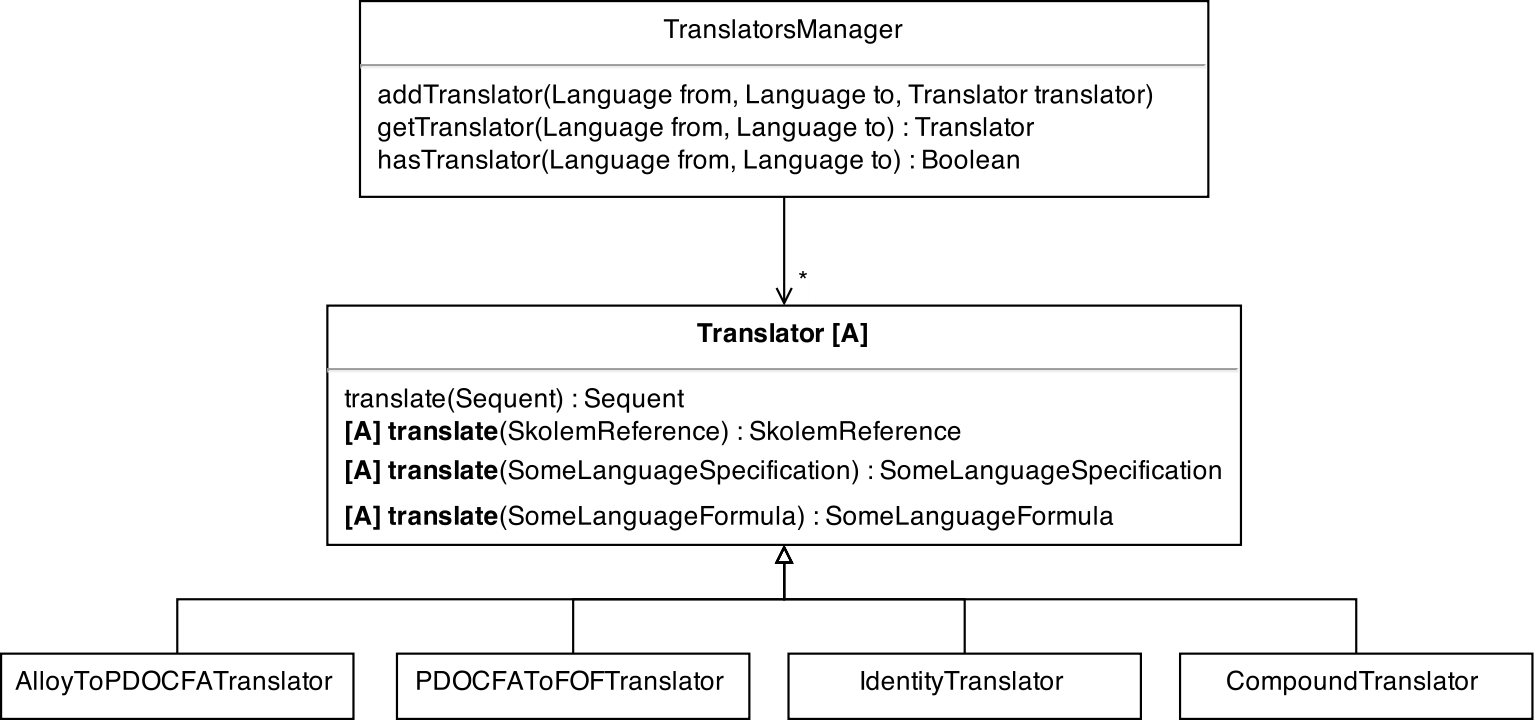
\includegraphics[width=400px]{img/arq_traductores.png}
\end{figure}

Se proveen los traductores de \textit{Alloy} a \textit{PDOCFA}, de \textit{PDOCFA} a \textit{TPTP-FOF} asi como el \textit{CompoundTranslator} que permite componer los traductores para lograr traducciones transitivas, por ejemplo de \textit{Alloy} a \textit{TPTP-FOF}.